
%% bare_jrnl.tex
%% V1.4
%% 2012/12/27
%% by Michael Shell
%% see http://www.michaelshell.org/
%% for current contact information.
%%
%% This is a skeleton file demonstrating the use of IEEEtran.cls
%% (requires IEEEtran.cls version 1.8 or later) with an IEEE journal paper.
%%
%% Support sites:
%% http://www.michaelshell.org/tex/ieeetran/
%% http://www.ctan.org/tex-archive/macros/latex/contrib/IEEEtran/
%% and
%% http://www.ieee.org/



% *** Authors should verify (and, if needed, correct) their LaTeX system  ***
% *** with the testflow diagnostic prior to trusting their LaTeX platform ***
% *** with production work. IEEE's font choices can trigger bugs that do  ***
% *** not appear when using other class files.                            ***
% The testflow support page is at:
% http://www.michaelshell.org/tex/testflow/


%%*************************************************************************
%% Legal Notice:
%% This code is offered as-is without any warranty either expressed or
%% implied; without even the implied warranty of MERCHANTABILITY or
%% FITNESS FOR A PARTICULAR PURPOSE! 
%% User assumes all risk.
%% In no event shall IEEE or any contributor to this code be liable for
%% any damages or losses, including, but not limited to, incidental,
%% consequential, or any other damages, resulting from the use or misuse
%% of any information contained here.
%%
%% All comments are the opinions of their respective authors and are not
%% necessarily endorsed by the IEEE.
%%
%% This work is distributed under the LaTeX Project Public License (LPPL)
%% ( http://www.latex-project.org/ ) version 1.3, and may be freely used,
%% distributed and modified. A copy of the LPPL, version 1.3, is included
%% in the base LaTeX documentation of all distributions of LaTeX released
%% 2003/12/01 or later.
%% Retain all contribution notices and credits.
%% ** Modified files should be clearly indicated as such, including  **
%% ** renaming them and changing author support contact information. **
%%
%% File list of work: IEEEtran.cls, IEEEtran_HOWTO.pdf, bare_adv.tex,
%%                    bare_conf.tex, bare_jrnl.tex, bare_jrnl_compsoc.tex,
%%                    bare_jrnl_transmag.tex
%%*************************************************************************

% Note that the a4paper option is mainly intended so that authors in
% countries using A4 can easily print to A4 and see how their papers will
% look in print - the typesetting of the document will not typically be
% affected with changes in paper size (but the bottom and side margins will).
% Use the testflow package mentioned above to verify correct handling of
% both paper sizes by the user's LaTeX system.
%
% Also note that the "draftcls" or "draftclsnofoot", not "draft", option
% should be used if it is desired that the figures are to be displayed in
% draft mode.
%
\documentclass[journal]{IEEEtran}
%
% If IEEEtran.cls has not been installed into the LaTeX system files,
% manually specify the path to it like:
% \documentclass[journal]{../sty/IEEEtran}

\usepackage{graphicx}
\usepackage{subfigure}
\usepackage[cmex10]{amsmath}
\usepackage{cite}

\usepackage{hyperref}
\usepackage{multirow}
\usepackage[all]{hypcap} % fix links to figs/tabs

\renewcommand{\arraystretch}{1.1} % make tables more readable



% Some very useful LaTeX packages include:
% (uncomment the ones you want to load)


% *** MISC UTILITY PACKAGES ***
%
%\usepackage{ifpdf}
% Heiko Oberdiek's ifpdf.sty is very useful if you need conditional
% compilation based on whether the output is pdf or dvi.
% usage:
% \ifpdf
%   % pdf code
% \else
%   % dvi code
% \fi
% The latest version of ifpdf.sty can be obtained from:
% http://www.ctan.org/tex-archive/macros/latex/contrib/oberdiek/
% Also, note that IEEEtran.cls V1.7 and later provides a builtin
% \ifCLASSINFOpdf conditional that works the same way.
% When switching from latex to pdflatex and vice-versa, the compiler may
% have to be run twice to clear warning/error messages.






% *** CITATION PACKAGES ***
%
%\usepackage{cite}
% cite.sty was written by Donald Arseneau
% V1.6 and later of IEEEtran pre-defines the format of the cite.sty package
% \cite{} output to follow that of IEEE. Loading the cite package will
% result in citation numbers being automatically sorted and properly
% "compressed/ranged". e.g., [1], [9], [2], [7], [5], [6] without using
% cite.sty will become [1], [2], [5]--[7], [9] using cite.sty. cite.sty's
% \cite will automatically add leading space, if needed. Use cite.sty's
% noadjust option (cite.sty V3.8 and later) if you want to turn this off
% such as if a citation ever needs to be enclosed in parenthesis.
% cite.sty is already installed on most LaTeX systems. Be sure and use
% version 4.0 (2003-05-27) and later if using hyperref.sty. cite.sty does
% not currently provide for hyperlinked citations.
% The latest version can be obtained at:
% http://www.ctan.org/tex-archive/macros/latex/contrib/cite/
% The documentation is contained in the cite.sty file itself.






% *** GRAPHICS RELATED PACKAGES ***
%
\ifCLASSINFOpdf
  % \usepackage[pdftex]{graphicx}
  % declare the path(s) where your graphic files are
  % \graphicspath{{../pdf/}{../jpeg/}}
  % and their extensions so you won't have to specify these with
  % every instance of \includegraphics
  % \DeclareGraphicsExtensions{.pdf,.jpeg,.png}
\else
  % or other class option (dvipsone, dvipdf, if not using dvips). graphicx
  % will default to the driver specified in the system graphics.cfg if no
  % driver is specified.
  % \usepackage[dvips]{graphicx}
  % declare the path(s) where your graphic files are
  % \graphicspath{{../eps/}}
  % and their extensions so you won't have to specify these with
  % every instance of \includegraphics
  % \DeclareGraphicsExtensions{.eps}
\fi
% graphicx was written by David Carlisle and Sebastian Rahtz. It is
% required if you want graphics, photos, etc. graphicx.sty is already
% installed on most LaTeX systems. The latest version and documentation
% can be obtained at: 
% http://www.ctan.org/tex-archive/macros/latex/required/graphics/
% Another good source of documentation is "Using Imported Graphics in
% LaTeX2e" by Keith Reckdahl which can be found at:
% http://www.ctan.org/tex-archive/info/epslatex/
%
% latex, and pdflatex in dvi mode, support graphics in encapsulated
% postscript (.eps) format. pdflatex in pdf mode supports graphics
% in .pdf, .jpeg, .png and .mps (metapost) formats. Users should ensure
% that all non-photo figures use a vector format (.eps, .pdf, .mps) and
% not a bitmapped formats (.jpeg, .png). IEEE frowns on bitmapped formats
% which can result in "jaggedy"/blurry rendering of lines and letters as
% well as large increases in file sizes.
%
% You can find documentation about the pdfTeX application at:
% http://www.tug.org/applications/pdftex





% *** MATH PACKAGES ***
%
%\usepackage[cmex10]{amsmath}
% A popular package from the American Mathematical Society that provides
% many useful and powerful commands for dealing with mathematics. If using
% it, be sure to load this package with the cmex10 option to ensure that
% only type 1 fonts will utilized at all point sizes. Without this option,
% it is possible that some math symbols, particularly those within
% footnotes, will be rendered in bitmap form which will result in a
% document that can not be IEEE Xplore compliant!
%
% Also, note that the amsmath package sets \interdisplaylinepenalty to 10000
% thus preventing page breaks from occurring within multiline equations. Use:
%\interdisplaylinepenalty=2500
% after loading amsmath to restore such page breaks as IEEEtran.cls normally
% does. amsmath.sty is already installed on most LaTeX systems. The latest
% version and documentation can be obtained at:
% http://www.ctan.org/tex-archive/macros/latex/required/amslatex/math/





% *** SPECIALIZED LIST PACKAGES ***
%
%\usepackage{algorithmic}
% algorithmic.sty was written by Peter Williams and Rogerio Brito.
% This package provides an algorithmic environment fo describing algorithms.
% You can use the algorithmic environment in-text or within a figure
% environment to provide for a floating algorithm. Do NOT use the algorithm
% floating environment provided by algorithm.sty (by the same authors) or
% algorithm2e.sty (by Christophe Fiorio) as IEEE does not use dedicated
% algorithm float types and packages that provide these will not provide
% correct IEEE style captions. The latest version and documentation of
% algorithmic.sty can be obtained at:
% http://www.ctan.org/tex-archive/macros/latex/contrib/algorithms/
% There is also a support site at:
% http://algorithms.berlios.de/index.html
% Also of interest may be the (relatively newer and more customizable)
% algorithmicx.sty package by Szasz Janos:
% http://www.ctan.org/tex-archive/macros/latex/contrib/algorithmicx/




% *** ALIGNMENT PACKAGES ***
%
%\usepackage{array}
% Frank Mittelbach's and David Carlisle's array.sty patches and improves
% the standard LaTeX2e array and tabular environments to provide better
% appearance and additional user controls. As the default LaTeX2e table
% generation code is lacking to the point of almost being broken with
% respect to the quality of the end results, all users are strongly
% advised to use an enhanced (at the very least that provided by array.sty)
% set of table tools. array.sty is already installed on most systems. The
% latest version and documentation can be obtained at:
% http://www.ctan.org/tex-archive/macros/latex/required/tools/


% IEEEtran contains the IEEEeqnarray family of commands that can be used to
% generate multiline equations as well as matrices, tables, etc., of high
% quality.




% *** SUBFIGURE PACKAGES ***
%\ifCLASSOPTIONcompsoc
%  \usepackage[caption=false,font=normalsize,labelfont=sf,textfont=sf]{subfig}
%\else
%  \usepackage[caption=false,font=footnotesize]{subfig}
%\fi
% subfig.sty, written by Steven Douglas Cochran, is the modern replacement
% for subfigure.sty, the latter of which is no longer maintained and is
% incompatible with some LaTeX packages including fixltx2e. However,
% subfig.sty requires and automatically loads Axel Sommerfeldt's caption.sty
% which will override IEEEtran.cls' handling of captions and this will result
% in non-IEEE style figure/table captions. To prevent this problem, be sure
% and invoke subfig.sty's "caption=false" package option (available since
% subfig.sty version 1.3, 2005/06/28) as this is will preserve IEEEtran.cls
% handling of captions.
% Note that the Computer Society format requires a larger sans serif font
% than the serif footnote size font used in traditional IEEE formatting
% and thus the need to invoke different subfig.sty package options depending
% on whether compsoc mode has been enabled.
%
% The latest version and documentation of subfig.sty can be obtained at:
% http://www.ctan.org/tex-archive/macros/latex/contrib/subfig/




% *** FLOAT PACKAGES ***
%
%\usepackage{fixltx2e}
% fixltx2e, the successor to the earlier fix2col.sty, was written by
% Frank Mittelbach and David Carlisle. This package corrects a few problems
% in the LaTeX2e kernel, the most notable of which is that in current
% LaTeX2e releases, the ordering of single and double column floats is not
% guaranteed to be preserved. Thus, an unpatched LaTeX2e can allow a
% single column figure to be placed prior to an earlier double column
% figure. The latest version and documentation can be found at:
% http://www.ctan.org/tex-archive/macros/latex/base/


%\usepackage{stfloats}
% stfloats.sty was written by Sigitas Tolusis. This package gives LaTeX2e
% the ability to do double column floats at the bottom of the page as well
% as the top. (e.g., "\begin{figure*}[!b]" is not normally possible in
% LaTeX2e). It also provides a command:
%\fnbelowfloat
% to enable the placement of footnotes below bottom floats (the standard
% LaTeX2e kernel puts them above bottom floats). This is an invasive package
% which rewrites many portions of the LaTeX2e float routines. It may not work
% with other packages that modify the LaTeX2e float routines. The latest
% version and documentation can be obtained at:
% http://www.ctan.org/tex-archive/macros/latex/contrib/sttools/
% Do not use the stfloats baselinefloat ability as IEEE does not allow
% \baselineskip to stretch. Authors submitting work to the IEEE should note
% that IEEE rarely uses double column equations and that authors should try
% to avoid such use. Do not be tempted to use the cuted.sty or midfloat.sty
% packages (also by Sigitas Tolusis) as IEEE does not format its papers in
% such ways.
% Do not attempt to use stfloats with fixltx2e as they are incompatible.
% Instead, use Morten Hogholm'a dblfloatfix which combines the features
% of both fixltx2e and stfloats:
%
% \usepackage{dblfloatfix}
% The latest version can be found at:
% http://www.ctan.org/tex-archive/macros/latex/contrib/dblfloatfix/




%\ifCLASSOPTIONcaptionsoff
%  \usepackage[nomarkers]{endfloat}
% \let\MYoriglatexcaption\caption
% \renewcommand{\caption}[2][\relax]{\MYoriglatexcaption[#2]{#2}}
%\fi
% endfloat.sty was written by James Darrell McCauley, Jeff Goldberg and 
% Axel Sommerfeldt. This package may be useful when used in conjunction with 
% IEEEtran.cls'  captionsoff option. Some IEEE journals/societies require that
% submissions have lists of figures/tables at the end of the paper and that
% figures/tables without any captions are placed on a page by themselves at
% the end of the document. If needed, the draftcls IEEEtran class option or
% \CLASSINPUTbaselinestretch interface can be used to increase the line
% spacing as well. Be sure and use the nomarkers option of endfloat to
% prevent endfloat from "marking" where the figures would have been placed
% in the text. The two hack lines of code above are a slight modification of
% that suggested by in the endfloat docs (section 8.4.1) to ensure that
% the full captions always appear in the list of figures/tables - even if
% the user used the short optional argument of \caption[]{}.
% IEEE papers do not typically make use of \caption[]'s optional argument,
% so this should not be an issue. A similar trick can be used to disable
% captions of packages such as subfig.sty that lack options to turn off
% the subcaptions:
% For subfig.sty:
% \let\MYorigsubfloat\subfloat
% \renewcommand{\subfloat}[2][\relax]{\MYorigsubfloat[]{#2}}
% However, the above trick will not work if both optional arguments of
% the \subfloat command are used. Furthermore, there needs to be a
% description of each subfigure *somewhere* and endfloat does not add
% subfigure captions to its list of figures. Thus, the best approach is to
% avoid the use of subfigure captions (many IEEE journals avoid them anyway)
% and instead reference/explain all the subfigures within the main caption.
% The latest version of endfloat.sty and its documentation can obtained at:
% http://www.ctan.org/tex-archive/macros/latex/contrib/endfloat/
%
% The IEEEtran \ifCLASSOPTIONcaptionsoff conditional can also be used
% later in the document, say, to conditionally put the References on a 
% page by themselves.




% *** PDF, URL AND HYPERLINK PACKAGES ***
%
%\usepackage{url}
% url.sty was written by Donald Arseneau. It provides better support for
% handling and breaking URLs. url.sty is already installed on most LaTeX
% systems. The latest version and documentation can be obtained at:
% http://www.ctan.org/tex-archive/macros/latex/contrib/url/
% Basically, \url{my_url_here}.




% *** Do not adjust lengths that control margins, column widths, etc. ***
% *** Do not use packages that alter fonts (such as pslatex).         ***
% There should be no need to do such things with IEEEtran.cls V1.6 and later.
% (Unless specifically asked to do so by the journal or conference you plan
% to submit to, of course. )


% correct bad hyphenation here
\hyphenation{op-tical net-works semi-conduc-tor}


\begin{document}
%
% paper title
% can use linebreaks \\ within to get better formatting as desired
% Do not put math or special symbols in the title.
\title{Applications of Many-Core Technologies to On-line Event Reconstruction in High Energy Physics
Experiments}
%
%
% author names and IEEE memberships
% note positions of commas and nonbreaking spaces ( ~ ) LaTeX will not break
% a structure at a ~ so this keeps an author's name from being broken across
% two lines.
% use \thanks{} to gain access to the first footnote area
% a separate \thanks must be used for each paragraph as LaTeX2e's \thanks
% was not built to handle multiple paragraphs
%


% note the % following the last \IEEEmembership and also \thanks - 
% these prevent an unwanted space from occurring between the last author name
% and the end of the author line. i.e., if you had this:
% 
% \author{....lastname \thanks{...} \thanks{...} }
%                     ^------------^------------^----Do not want these spaces!
%
% a space would be appended to the last name and could cause every name on that
% line to be shifted left slightly. This is one of those "LaTeX things". For
% instance, "\textbf{A} \textbf{B}" will typeset as "A B" not "AB". To get
% "AB" then you have to do: "\textbf{A}\textbf{B}"
% \thanks is no different in this regard, so shield the last } of each \thanks
% that ends a line with a % and do not let a space in before the next \thanks.
% Spaces after \IEEEmembership other than the last one are OK (and needed) as
% you are supposed to have spaces between the names. For what it is worth,
% this is a minor point as most people would not even notice if the said evil
% space somehow managed to creep in.

% paper title
\title{Applications of Many-Core Technologies to On-line Event Reconstruction in High Energy Physics
Experiments}
% Author list
\author{A.~Gianelle, 
  S.~Amerio, 
  D.~Bastieri, 
  M.~Corvo, 
  W.~Ketchum,
  T.~Liu, 
  A.~Lonardo, 
  D.~Lucchesi,
  S.~Poprocki, 
  R.~Rivera, 
  L.~Tosoratto,
  P.~Vicini
  and 
  P.~Wittich
\thanks{Manuscript received XXX, XXX.
This work was supported by the  US National Science Foundation, the US 
Department of Energy Office of Science and the Italian
Istituto Nazionale di Fisica Nucleare. This work was partially supported by the 
EU Framework Programme 7 project EURETILE under grant number 247846.}% <-this % stops a space
\thanks{D.~Bastieri and D.~Lucchesi are with University of Padova and INFN Padova.}% 
\thanks{A.~Gianelle is with INFN Padova.}% 
\thanks{M.~Corvo is with University of Ferrara.}% 
\thanks{S.~Amerio is with University of Padova.}% 
\thanks{W.~Ketchum is with Los Alamos National Laboratory.}%
\thanks{T.~Liu and R.~Rivera are with Fermi National Accelerator Laboratory.}%
\thanks{A.~Lonardo, L.~Tosoratto and P.~Vicini are with INFN Roma.}% 
\thanks{S.~Poprocki and P.~Wittich are with Cornell University.}
}

% The paper headers
%\markboth{Journal of \LaTeX\ Class Files,~Vol.~11, No.~4, December~2012}%
%{Shell \MakeLowercase{\textit{et al.}}: Bare Demo of IEEEtran.cls for Journals}
% The only time the second header will appear is for the odd numbered pages
% after the title page when using the twoside option.
% 
% *** Note that you probably will NOT want to include the author's ***
% *** name in the headers of peer review papers.                   ***
% You can use \ifCLASSOPTIONpeerreview for conditional compilation here if
% you desire.




% If you want to put a publisher's ID mark on the page you can do it like
% this:
%\IEEEpubid{0000--0000/00\$00.00~\copyright~2012 IEEE}
% Remember, if you use this you must call \IEEEpubidadjcol in the second
% column for its text to clear the IEEEpubid mark.



% use for special paper notices
%\IEEEspecialpapernotice{(Invited Paper)}




% make the title area
\maketitle

% As a general rule, do not put math, special symbols or citations
% in the abstract or keywords.
\begin{abstract}
The abstract goes here.
\end{abstract}

% Note that keywords are not normally used for peerreview papers.
%\begin{IEEEkeywords}
%IEEEtran, journal, \LaTeX, paper, template.
%\end{IEEEkeywords}






% For peer review papers, you can put extra information on the cover
% page as needed:
% \ifCLASSOPTIONpeerreview
% \begin{center} \bfseries EDICS Category: 3-BBND \end{center}
% \fi
%
% For peerreview papers, this IEEEtran command inserts a page break and
% creates the second title. It will be ignored for other modes.
\IEEEpeerreviewmaketitle



\section{Introduction}
\IEEEPARstart{R}{eal}-time event reconstruction plays a fundamental role in High Energy
Physics (HEP) experiments at hadron colliders.  Reducing the rate of
data to be saved on tape is critical. To increase the purity of the collected samples,
rate reduction has to be coupled with an initial selection of the most
interesting events.  In a typical hadron collider experiment, the
event rate has to be reduced from tens of MHz to a few kHz.  The
selection system (trigger) is usually organized in successive levels,
each capable of performing a finer selection on more complex physics
objects describing the event. Trigger systems usually comprise a first
level based on custom hardware, followed by one or two levels usually
based on farms of general purpose processors.  At all levels, latency
is a concern: for a fixed processing time, the faster a decision is
rendered about accepting or rejecting an event improves the purity of
the collected data sample. The possibility of using commercial devices
at a low trigger level is very appealing: they are subject to
continuous performance improvements driven by the consumer market, are
less expensive than dedicated hardware, and are easier to support.
Among the commercial devices, many-core architectures such as Graphic
Processing Units (GPUs)~\cite{bib_gpu} and Intel Many Integrated Core
(MIC)~\cite{bib_intelMIC} are of particular interest for online
selections given their great computing power: the latest
\textsc{nvidia}~\cite{bib_nvidia} GPU architecture, Kepler, exceeds
Teraflop computing power. Moreover, high-level programming
architectures based on \textsc{c/c++} such as
\textsc{cuda}~\cite{bib_cuda} and \textsc{opencl}~\cite{bib_opencl}
make programming these devices more accessible to the general
physicist user.  The goal of this study is to investigate the
strengths and weaknesses of many-core devices when applied in a low
latency environment, with particular emphasis on the data transfer
latency to/from the device and the algorithm latency for processing on
the device in a manner similar to a typical HEP trigger application,
and to understand the cost/complexity ratio of porting legacy serial
code to many-core devices.

We showed initial studies on GPU performance in low-latency
environments ($\approx 100~\mu$s) in previous
papers~\cite{TIPP2011,NSS2012,CHEP2013}.  In this paper we extend
those studies to include other many-core architectures (Intel MIC 
and \textsc{amd} GPUs in
addition to \textsc{nvidia} GPUs) and other programming 
toolsets (\textsc{opencl} in addition to \textsc{cuda}).
The algorithm run on the parallel architecture is a complete version
of the fast track-fitting algorithm of the Silicon Vertex Tracker
(SVT) system at CDF~\cite{SVT1}.  
%We also investigate the performance
%of the algorithm on a GPU manufactured by AMD using a different
%computing environment: \textsc{opencl}.  
Starting with a serial algorithm implemented on a CPU, 
we test an \textit{embarrassingly
  parallel} algorithm on the Intel MIC environment. In this case each
event is handled independently by a core on the accelerator, and the
parallelization is achieved with only minor changes to the legacy
code.  This approach is only possible in the Intel MIC
environment. Next we consider an algorithm where we unroll three
internal nested loops and run these in parallel on a GPU, using the
\textsc{cuda} and \textsc{opencl} environments. This second approach
is programmatically more complicated and less trivial to implement. In
neither case have we re-thought the basic algorithms or the data
structures used. To achieve optimal performance, these steps would
have to be taken.  As one might expect, the improvement from the first
approach is rather modest, albeit easier to implement, and the second
approach shows larger performance gains. For GPUs, we also test
different strategies to transfer data to and from the device.

\section{SVT track fitting algorithm}
The Silicon Vertex Trigger (SVT)~\cite{SVT1,SVT2} is a track
reconstruction processor used in the CDF experiment at Tevatron
accelerator. It reconstructs tracks in about 20 $\mu s$ in two steps:
first, low resolution tracks (\textit{roads}) are found in each event
among the energy deposits left in the tracking detector by charged
particles; second, track fitting is performed on all possible
combinations of hits inside a road.  This algorithm uses a linearized
approximation to track-fitting as implemented in hardware (described
in greater detail in~\cite{SVT3}).  With the linearized track fit of
the SVT approach, the determination of the track parameters ($p_i$) is
reduced to a simple scalar product:
\[
p_i = \vec{f_i} \cdot \vec{x_i} + q_i,
\]
where $\vec{x_i}$ are input silicon hits, and $\vec{f_i}$ and $q_i$ are 
pre-defined constant sets. For each set of hits, the algorithm
computes the impact parameter $d_0$, the azimuthal angle $\phi$, 
the transverse momentum $p_\mathrm{T}$ , and the $\chi^2$ of the
fitted track by using simple operations such as memory lookup and 
integer addition and multiplication.

We ported the track fitting as it is well suited to parallelization -
each track can be handled independently.

\subsection{Code implementation}
The starting point of our studies is the SVT track fitting
simulation code, written in the \textsc{c} language. SVT track fitting
is divided into three main functions: first, the unpacking of input
data and filling of all the necessary data structures; second, the
computation of all possible combinations of hits in each road and
third, the linearized track fit of each combination of hits. Three
main loops are present - on events, roads and hit combinations.

To be run on \textsc{nvidia} GPUs, the code has been ported to \textsc{cuda}:
each step -- unpack, combine and track fit -- is performed by a
specific kernel; the three nested loops are unrolled so that each GPU
thread processes a single combination of hits.  The \textsc{cuda}
implementation makes use of \textsc{thrust}~\cite{bib_thrust}, a C++
template library for \textsc{cuda}, in the unpacking step. The
existence of template libraries such as \textsc{thrust} is an
advantage of the \textsc{cuda} environment.

To implement the algorithm to run on an \textsc{amd} GPU, we have ported the
\textit{combine} and \textit{track fit} \textsc{cuda} kernels to
\textsc{opencl}, which requires minimal changes. Because the
\textsc{thrust} template libraries can only be used with
\textsc{cuda}, we resort to unpacking serially on the CPU.

To run on MIC, where cores are more powerful but fewer in number, we
adopted the so-called \textit{embarrassingly parallel} approach and
used \textsc{pragma OpenMP} for statements to unroll only the external
loop on the events, so that each core processes a single event: the
porting requires much less effort compared to \textsc{cuda}, but the
level of parallelism is limited.


\subsection{Experimental setups}
The many-core devices used in this study are listed in
Table~\ref{tab_hwspecs}. The GPUs include a less expensive gaming
class GPUs (the \textsc{nvidia} GTX and \textsc{amd} Radeon cards) and ones optimized
for scientific computing (Tesla). The MIC corresponds to a Xeon Phi
introduced in November 2012.

\begin{table*}[tbp]
  \caption{Capabilities of the many-core devices used in this study,
    according to the manufacturer's specifications. The first three
    are \textsc{nvidia} GPUs, the MIC 5110P is an Intel Xeon Phi, and
    the final one is an \textsc{amd} GPU.  For Xeon Phi, the ``cores'' column
    counts the HW threads per core as equivalent to a GPU core.}
  \label{tab_hwspecs}
  \centering
  \begin{tabular}{|l|c|c|c|c|c|}
    \hline
    Model & Tesla M2050 & Tesla K20m & GeForce GTX  Titan & MIC 5110P & Radeon HD 7970 \\
    \hline
     \hline
    Performance (SP, GFlops) & 1030 & 3520 & 4500 & 2022 & 3790\\
    Memory bandwidth  (GB/s) & 148 & 208 & 288  & 320 & 264\\   
    Memory size (GB) & 3 & 5 & 6 & 8 & 3\\
    Number of cores & 448 & 2496 & 2688 & 240 & 2048\\
    Clock speed (GHz) & 1.15 & 0.706 & 0.837 & 1.053 & 1.375\\
    \hline
  \end{tabular}
\end{table*}

To measure the data transfer latency we use a computing cluster composed of 
12 identical nodes.  Each node contains a Intel Xeon E6520 2.4 GHz 
CPU and two Tesla M2075 GPU cards. The nodes are connected by InfiniBand 
communication links using Connect-X2 Mellanox or APEnet+ adapters. 
APEnet+ is an FPGA-based PCIe board supporting peer-to-peer communication with 
Tesla and Kepler cards~\cite{apenet2010}.
Two nodes of this cluster are used to measure data transfer latency,
one acting as a transmitter and the
other as a receiver.  Data are transferred from the transmitter to the 
receiver, processed on the GPU and sent back to the receiver (see
Fig.~\ref{fig:data_flow}).  
The latency for a complete loop is measured on the transmitter using 
standard \textsc{c} libraries.
\begin{figure}[tbp]
\centering
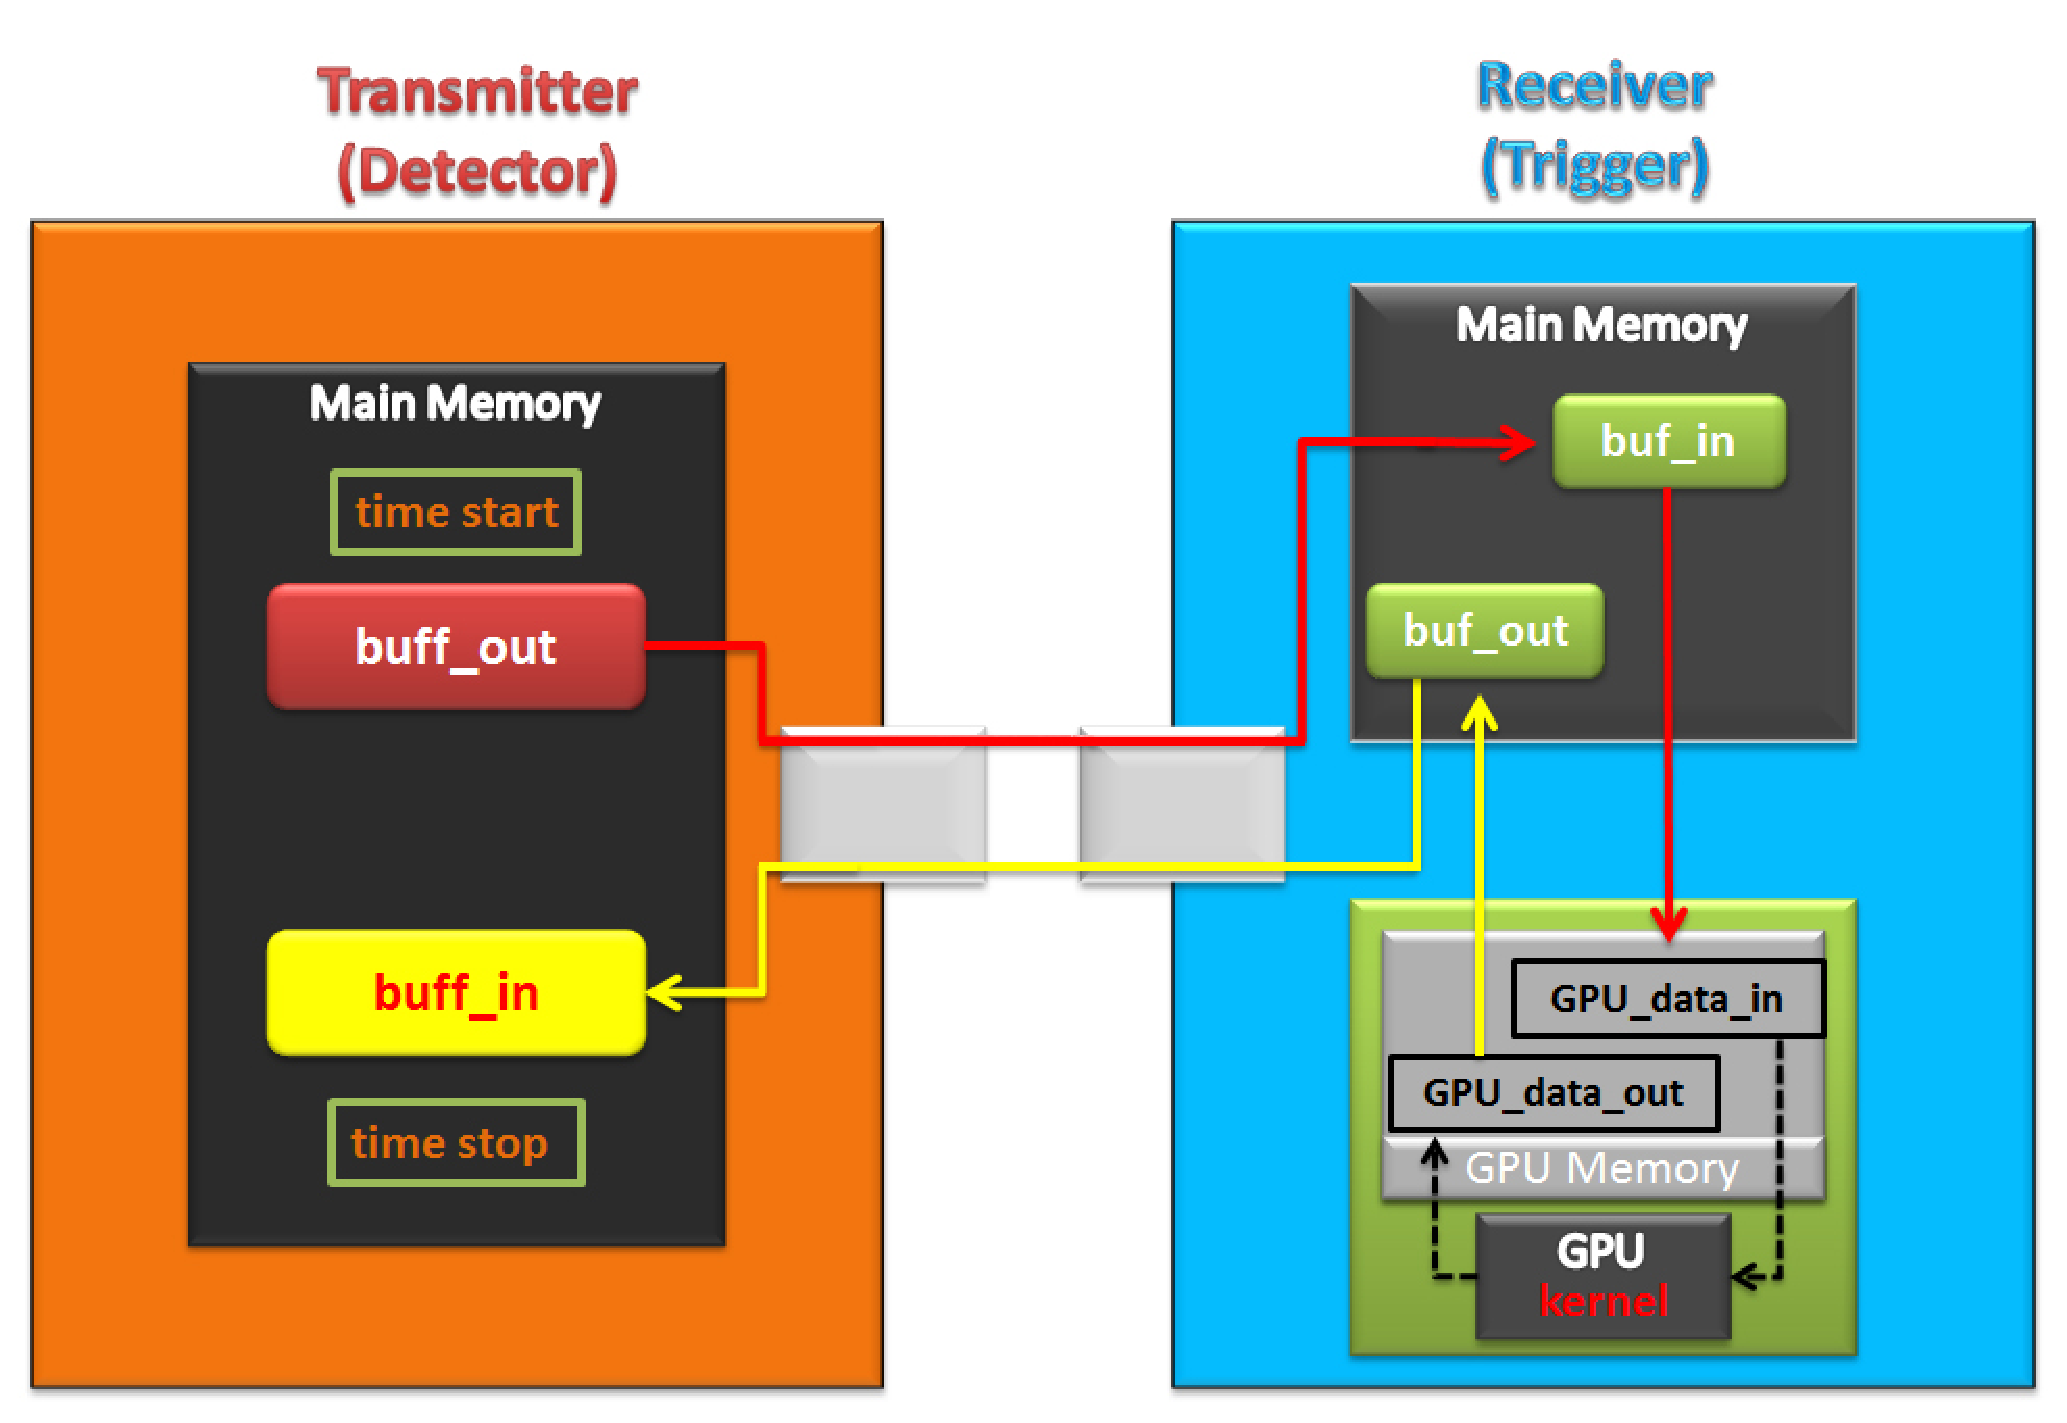
\includegraphics[width=3.5in]{figures/SetUp-general}
\caption{Data flow. Data is sent from the transmitter PC to the
  receiver PC, where it is processed by the GPU before being returned
  to the transmitter PC. The transmitter plays the role of the
  detector as the source of the data and as an upstream trigger
  processor as the data's ultimate sink. The receiver PC plays the
  role of a component in the trigger system. }
\label{fig:data_flow}
\end{figure}
In this setup, the transmitter can represent the detector, as
the source of the data, or an upstream trigger processor, as
the ultimate sink of the data, while the receiver is the
trigger system: the time to transfer data to the receiver is thus a
rough estimate of the latency to transfer the data from the detector
front-end to the trigger system.

We have an additional setup for testing the \textsc{opencl}
implementation of the track fitting algorithm. Here, we use a 3.07 GHz
Intel Core i7 CPU 950, which has four cores and up to eight
computation threads. We run the algorithm serially on this CPU (one
core), and also run a CPU-based \textsc{opencl} algorithm which makes
use of the multi-core architecture. Additionally, we have an \textsc{amd}
Radeon HD 7970 GPU in a PCIe slot in this setup, on which we also run
the \textsc{opencl} algorithm.

The power measurements are performed on a \textsc{cuda} development kit~\cite{bib_kayla} 
based on the kayla MITX platform. This kit features a  
\textsc{nvidia} Tegra 3 \textsc{arm} Cortex A9 Quad-Core and a Quadro K2000 GPU, both low
energy consumption devices.

\section{Results}
The input data consists of events with a fixed number of roads and
combinations: each event has 2048 combinations to be fitted. To
explore different data-taking conditions, the number of events ranges
from one to 3000, \emph{i.e.,} between 2048 to about six millions of
combinations to fit.

\subsection{Data processing results}
Each data sample is processed 100 times by the track fitting algorithm. 
The average latency as a function of the number of fits is presented in 
Fig.~\ref{fig:algo_only_timing} for the serial,
embarrassingly parallel and parallel algorithms. We see that the
embarrassingly parallel algorithm gives a modest increase with respect
to the serial (CPU) algorithm. Switching to a fully parallel algorithm
affords a much more significant speed improvement. 
\begin{figure}[!t]
  \centering
  \includegraphics[width=0.9\linewidth]{figures/TimeComp_MIC}
  \caption{Algorithm-only comparison for timing as a function of the
    number of track fits. We compare timing on CPUs (serial), Intel
    MIC (embarrassingly parallel), and GPUs (fully parallel), in
    blue, green, and red, respectively. The GPUs exhibit the best
    performance due to the full parallelization. }
  \label{fig:algo_only_timing}
\end{figure}
\begin{figure}[!t]
  \centering
  \includegraphics[width=0.9\linewidth]{figures/TimeCompZoom_MIC.png} 
  \caption{Algorithm-only comparison for timing as a function of the
    number of track fits: zoom in the low number of fits region. At
    low number of fits, the CPU performs better, due to start-up
    costs associated with data transfers to the accelerator card.}
  \label{fig:algo_only_timing_zoom}
\end{figure}
\begin{figure}[!t]
  \centering
  \includegraphics[width=0.9\linewidth]{figures/Speedup_MIC}
  \caption{Speed-up with respect to a standard CPU (Intel Xeon
    E5630). The speed-ups plateau after about two million fits.}
  \label{fig:algo_only_speedup}
\end{figure}
The accelerator card's performance drop with decreasing number of fits, as can be seen 
in Fig.~\ref{fig:algo_only_timing_zoom}, due to overhead.
Figure~\ref{fig:algo_only_speedup} shows the speed-up with respect to the serial 
algorithm run on a standard CPU (Intel Xeon E5630): the maximum gain is 
obtained processing at least 500 events. This means that to fully exploit 
parallel architectures millions of fits have to be performed in parallel.

\subsubsection{Breakdown of computing time}
In Fig.~\ref{fig:breakdown} we show the fractional time spent in
various parts of the algorithm for the embarrassingly parallel algorithm 
(on Intel MIC) and the parallel algorithm (on \textsc{nvidia} Titan GPU), as a 
function of the number of fits. On both accelerator cards the fractional times
are constant for more than 500 input events, where computing resources are saturated. 
Unlike the MIC, the fit stage takes most of the time on the GPU: this 
could be caused by the intense memory access frequency intrinsic to
this part of the algorithm.  
\begin{figure*}[!t]
\centering
\subfigure[]
{\label{fig:breakdown_MIC}
\includegraphics[width=0.45\linewidth]{figures/Mic5_perc_nk}}
\subfigure[]
{\label{fig:breakdown_GPU}
\includegraphics[width=0.45\linewidth]{figures/titan_perc}}
\caption{Breakdown of computing time for MIC (a) and the GTX Titan GPU
  (b). White corresponds to unpacking, green hash corresponds to
  generating hit combinations, solid blue is the linearized track fit,
  and magenta cross-hatch corresponds to offloading (MIC only). For
  MIC, combinations and fitting take the same amount of time for large
  number of events. For GPU, fitting dominates. }
\label{fig:breakdown}
\end{figure*}


\subsubsection{Data processing in \textsc{opencl}}
We also measure the track fitting algorithm latency in an
implementation using \textsc{opencl}. The \textsc{opencl} tools have
the advantage of being an open standard, while the \textsc{cuda} tools
are only compatible with \textsc{nvidia} GPUs. Additionally, \textsc{opencl}
can work also on CPUs and on the Xeon Phi. For our tests, due to
limitations on the available space for storing data on the GPU, we
only test the algorithm on up to 1000 events (\textit{i.e.} about 2
million combinations to fit). In Fig.~\ref{fig:opencl_timing} we show
the results of algorithm latency measurements for three different
modes: running the serial algorithm on the CPU (single-core), running
the \textsc{opencl} algorithm on the CPU (multi-core), and running the
\textsc{opencl} algorithm on the \textsc{amd} Radeon GPU. The \textsc{opencl}
implementation of the algorithm on the CPU provides a significant
speedup---about a factor of 5---over running the algorithm serially on
the CPU. Running the same \textsc{opencl} algorithm on the GPU
provides an even greater speedup due to the increased number of cores
and parallel threads that can be run, though there is additional
latency to copy data into and out of the GPU that makes running on the
GPU take longer for small numbers of combinations to fit.
\begin{figure}[!t]
  \centering
  \includegraphics[width=0.9\linewidth]{figures/openclamd.pdf}
  \caption{The timing of the \textsc{opencl} algorithm as a function of the
    number of track fits. We compare timing running the algorithm serially on a CPU, 
    using \textsc{opencl} on the CPU, and on an \textsc{amd} GPU.}
  \label{fig:opencl_timing}
\end{figure}
Surprisingly, though \textsc{opencl} is an open standard, we find that
we are unable to run the same \textsc{opencl} code on \textsc{nvidia} GPUs. On two
different installations with two different video cards, we find
incorrect results running the code that ran successfully on the \textsc{amd}
card. At present it is unclear what the root cause  is.

\subsection{Data processing vs power consumption}

\begin{table*}[tbp]
  \caption{}
  \label{tab_kayla}
  \centering
  \begin{tabular}{|l|c|c|c|}
    \hline
         & \multicolumn{3}{|c|}{Absorbed current (A)} \\
    \hline
    Mode & ARM & GPU & Motherboard  \\
    \hline    
    \hline
    idle & 0.29 & 0.60-0.70 & 0.60 \\
    \hline
    read & 0.29 & 1.01  & 0.60 \\
    \hline
    Host $\rightarrow$ Device & 0.33 & 1.08  & 1.17 \\
    \hline
    Device $\rightarrow$ Host & 0.33 & 1.06  & 1.14 \\
    \hline
    Full algorithm & 0.33 & 0.98  & 2.24 \\
%    \hline
%    Full algorithm (no Thrust) & 0.33 & 1.06-1.08  & 1.15 \\
    \hline
  \end{tabular}
\end{table*}


\subsection{Data transfer}
The experimental setup described in Fig.~\ref{fig:data_flow} allows us to 
test different data transfer  strategies to the GPU. The standard data transfer 
strategy is via the system memory, where the 
PCIe adapter card and the GPU allocate \emph{separate} buffers on the
system memory for the copy (as shown in Fig.~\ref{fig:standardDT}).
This is inefficient, as the data are copied twice in the 
system memory before being transferred to the GPU/PCIe card. 
Data may also be transferred using Direct Memory Access (DMA, 
GPUDirect~\cite{bib_GPUDirect}) to the CPU memory:
the PCIe card and the GPU share the \textit{same} buffer on the CPU memory; as 
a result the data are copied only once in the CPU memory 
(Fig.~\ref{fig:GPUDirectV1}). 
With our experimental setup two additional copy strategies can be tested
which are the results of different levels of 
optimization of the GPUDirect protocol:
\begin{itemize}
\item \textsc{cuda}-Aware MPI, where the copy latency is further reduced
by automatically allocating the buffer on the CPU memory;
\item peer-to-peer (P2P) strategy, when data are transferred 
directly to the GPU, without any  
intermediate copy to the CPU (Fig.~\ref{fig:GPUDirectV2}).
\end{itemize}


\begin{figure*}[!t]
\centering
\subfigure[]
{\label{fig:standardDT}
\includegraphics[width=0.3\linewidth]{figures/noGPUDirect}}
\hspace{1mm}
\subfigure[]
{\label{fig:GPUDirectV1}
\includegraphics[width=0.3\linewidth]{figures/GPUDirect}}
\subfigure[]
{\label{fig:GPUDirectV2}
\includegraphics[width=0.3\linewidth]{figures/GPUDirect-APE}}
\caption{Standard data transfer (a), via GPUDirect (b) and via
  GPUDirect with P2P support (c). In (a), two buffers are required in
  the main memory. In GPUDirect (b), one of the main memory buffers is
  eliminated. In GPUDirect with P2P support, data is sent directly
  from the APEnet+ transceiver to the GPU memory.}
\end{figure*}

\begin{figure}[!t]
  \centering
  \includegraphics[width=0.85\linewidth]{figures/datatransfer}
  \caption{Total latency (data transfer, copy to/from the GPU and data
    processing on the GPU) as a function of data buffer sizes, for
    three different levels of optimization of GPUDirect: v1.0,
    \textsc{cuda}-aware MPI and P2P. The smallest transferred data
    packed is 600 kB.  \textsc{cuda}-aware MPI shows the best
    performance for larger packet size.}
  \label{fig:xferlatency}
\end{figure}

In Fig.~\ref{fig:xferlatency} we show the total latency (data
transfer, copy to/from the GPU and data processing on the GPU) as a
function of data packet size when data are transferred using GPUDirect
v1.0, \textsc{cuda}-aware MPI and P2P. For the packet sizes considered in this test 
 \textsc{cuda}-aware MPI gives the best performance. This is expected as 
P2P is optimized for small packet sizes
 (see also~\cite{NSS2012} and~\cite{bib_mvapich}). As a matter of fact, for larger packet size, the channel 
throughput becomes dominant: the shortest transfer 
time of CUDA aware-MPI system is easily explained comparing the link bandwidth of Mellanox board (40 Gb/s) 
with the smaller throughput of a APEnet+ single link (30 Gb/s).  
The data transfer latency accounts for a significant part of the total
latency, as can be seen in Fig.~\ref{fig:transferOnly}: about 20-25\%
of total latency is due to moving the data to and from the GPU.

\begin{figure}[!t]
  \centering
  \includegraphics[width=0.85\linewidth]{figures/cudaware}
  \caption{Time per fit, in msec. The two curves show total timing
    with and without calculations performed on the GPU, thereby
    showing the considerable time spent in data transfer. About
    20-25\% of the time is spent in data transfer.}
  \label{fig:transferOnly}
\end{figure}


\section{Conclusion}
The conclusion goes here.





% if have a single appendix:
%\appendix[Proof of the Zonklar Equations]
% or
%\appendix  % for no appendix heading
% do not use \section anymore after \appendix, only \section*
% is possibly needed

% use appendices with more than one appendix
% then use \section to start each appendix
% you must declare a \section before using any
% \subsection or using \label (\appendices by itself
% starts a section numbered zero.)
%


% use section* for acknowledgement
\section*{Acknowledgment}


The authors would like to thank...


% Can use something like this to put references on a page
% by themselves when using endfloat and the captionsoff option.
\ifCLASSOPTIONcaptionsoff
  \newpage
\fi



% trigger a \newpage just before the given reference
% number - used to balance the columns on the last page
% adjust value as needed - may need to be readjusted if
% the document is modified later
%\IEEEtriggeratref{8}
% The "triggered" command can be changed if desired:
%\IEEEtriggercmd{\enlargethispage{-5in}}

% references section

% can use a bibliography generated by BibTeX as a .bbl file
% BibTeX documentation can be easily obtained at:
% http://www.ctan.org/tex-archive/biblio/bibtex/contrib/doc/
% The IEEEtran BibTeX style support page is at:
% http://www.michaelshell.org/tex/ieeetran/bibtex/
%\bibliographystyle{IEEEtran}
% argument is your BibTeX string definitions and bibliography database(s)
%\bibliography{IEEEabrv,../bib/paper}
%
% <OR> manually copy in the resultant .bbl file
% set second argument of \begin to the number of references
% (used to reserve space for the reference number labels box)

\bibliographystyle{IEEEtran}

\bibliography{gpu}


% that's all folks
\end{document}


